\documentclass[palatino,nosec,nobuildate]{Docencia}


\title{Solución examen final}

\author{Departamento de Matemáticas}
\date{17/18}


% Paquetes adicionales

\usepackage[author={Víctor de Juan, 2017}]{pdfcomment}

\usepackage{pgf,tikz}
\usetikzlibrary{arrows}


\definecolor{qqttcc}{rgb}{0,0.2,0.8}
\definecolor{qqqqff}{rgb}{0,0,1}
\definecolor{cccccc}{rgb}{0.8,0.8,0.8}


\makeatletter
\newcommand{\annotate}[2][]{%
\pdfstringdef\x@title{#1}%
\edef\r{\string\r}%
\pdfstringdef\x@contents{#2}%
\pdfannot
width 2\baselineskip
height 2\baselineskip
depth 0pt
{
/Subtype /Text
/T (\x@title)
/Contents (\x@contents)
}%
}
\makeatother



\usepackage{eso-pic}
\newcommand\BackgroundPic{%
\put(0,0){%
\parbox[b][\paperheight]{\paperwidth}{%
\vfill
\centering

\includegraphics[width=\paperwidth,height=\paperheight,%
keepaspectratio]{../../../../BWLogo.jpeg}%
\vfill
}}}





\begin{abstract}
Solución del examen final de la segunda evaluación.

\nota{Estos ejemplos no están exentos de erratas. En caso de descubrir alguna, por favor, comunicarlas.}
\end{abstract}

% --------------------
\newcommand{\cimplies}{\text{\hl{$\implies$}}}

\begin{document}
\pagestyle{plain}
\maketitle

\AddToShipoutPicture{\BackgroundPic}

\begin{problem} (1.5 puntos)
Resuelve el siguiente sistema:

\[
	\left\{
		\begin{array}{c}
			\frac{3x+10}{2-x}≥1\\
			x^2-6x+9 ≥ 0
		\end{array}
	\right\}
\]
\solution

Resolvemos por separado cada una de ellas:

\[
	\frac{3x+10}{2-x}≥1 \dimplies \frac{3x+10}{2-x}-1≥0 \dimplies \frac{3x+10-2+x}{2-x}≥ 0 \dimplies \frac{4x+8}{2-x}≥0 
\]
Cuya solución, haciendo la tabla es: $(-∞,-2] ∪ (2,∞)$

\[
	x^2-6x+9 ≥ 0 \dimplies (x-3)^2 ≥ 0 \dimplies x\in(-∞,∞)
\]

La solución del sistema será: $\left((-∞,-2] ∪ (2,∞)\right)∩(-∞,∞) = (-∞,-2] ∪ (2,∞)$

\end{problem}

\begin{problem} (2 puntos)

Calcular la altura del rectángulo más alto y el área del triángulo.

\solution

\begin{figure}[h]
\centering
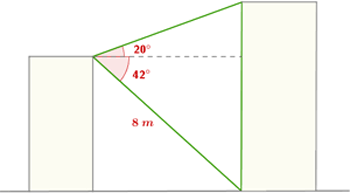
\includegraphics[scale=0.5]{prob.png}
\end{figure}

Utilizando la definición de $\sin(α)$ vamos a calcular la altura del rectángulo pequeño, $h_p$.

\[\sin(42) = \frac{h_p}{8} \implies h_p = 8·\sin(42)m\]

Necesitamos calcular la altura que falta del rectángulo grande. Para ello, necesitamos algún dato más del triángulo superior. Por ello, utilizando la definición de $\cos(α)$, podemos calcular la separación de los rectángulos $s_r$ (que es además la altura del triángulo).

\[
	\cos(42) = \frac{s_r}{8} \implies s_r = 8·\cos(42)m
\]

Ahora ya podemos calcular la altura restante $h_r$ utilizando la definición de $\tan(α)$.

\[
	\tan(20) = \frac{h_r}{s_r} \implies h_r = s_r·\tan(20) = 8·\cos(42)·\tan(20)m
\]

Por lo tanto, la altura del rectángulo grande será $h_T = h_p+h_r = 8·\sin(42)+8·\cos(42)·\tan(20)m$

Y el área:

\[
	A = \frac{b·h}{2} = \frac{h_t·s_r}{2} = \frac{\left(8·\sin(42)+8·\cos(42)·\tan(20)\right)·8·\cos(42)}{2}m^2
\]

Operando con la calculadora obtenemos los resultados finales.

\end{problem}

\begin{problem}(1,5 puntos) Determinar la ecuación general de la recta que pasa por el punto $A(-1,3)$ y:

\ppart $B(2,-6)$

\ppart Es paralela a la recta $r:2x-5y+3=0$

\ppart Es perpendicular a la recta $s: y=-3x$

\solution

\spart Utilizamos la ecuación continua de la recta. Para ello calculamos $\vec{[AB]} = (2-(-1),-6-3) = (3,-9)$

\[
	\frac{x-a_1}{v_1} = \frac{y-a_2}{v_2} \dimplies \frac{x+1}{3} = \frac{y-3}{-9}
\]

Operamos hasta obtener la ecuación general:
\[
 \frac{x+1}{3} = \frac{y-3}{-9} \dimplies -9(x+1) = 3(y-3) \dimplies -9x-3y=0\dimplies y=3x
\]

\spart La recta buscada será de la forma $2x-5y+k=0$, ya que así se cumple el criterio de paralelismo $\rfrac{A}{A'} = \rfrac{B}{B'}$.
%
Ahora calculamos el valor de $k$ para que la recta pase por el punto $A$.

\[
	2·(-1) - 5·(3) + k = 0 \dimplies k = 17
\]

La recta es:

\[
	2x-5y+17=0
\]

\spart La recta buscada tendrá pendiente $m = \rfrac{1}{3}$, ya que 2 rectas son perpendiculares si el producto de sus pendientes es $-1$. En este caso, $-3·\rfrac{1}{3} = -1$.

La recta buscada será de la forma: $y=\rfrac{1}{3}x + n$. Hallamos el valor de $n$ para que la recta pase por el punto $A$:

$3 = \frac{1}{3}·1 + n \dimplies n=3-\rfrac{1}{3} = \rfrac{8}{3}$

La recta es:

\[
	y=\frac{1}{3}x+\frac{8}{3}
\]

\end{problem}

\begin{problem} (1,5 puntos) Determinar el vector director y la pendiente de cada una de las rectas siguientes:

\ppart $5x-3y+1=0$

\ppart $\frac{4x+4}{2} = \frac{-y}{5}$

\ppart $\left\{\begin{array}{c} x=1-3t\\y=2\end{array}\right.$
\solution

\spart $\vec{v} = (-B,A) = (-(-3),5) = (3,5)$ y $m=\frac{v_2}{v_1} = \frac{5}{3}$

\spart La ecuación dada no es una ecuación conocida. Busco transformarla en una ecuación conocida. 

\[\frac{4x+4}{2} = \frac{-y}{5} \dimplies 20x+20+2y=0 \dimplies y=-10x-10\]

La pendiente es $m=-10$ y su vector director $\vec{v} = (1,m) = (1,-10)$

\spart El vector director es $\vec{v} = (1,0)$ ya que la recta es horizontal al tener siempre la misma coordenada $y$.

\end{problem}

\textit{Elegir uno de los 2 siguientes}
\begin{problem}
\ppart Hallar la ecuación general de la mediatriz del segmento $A(-2,0), B(4,-2)$.

\ppart Un candado $A$ tiene claves de 3 letras consonantes (en total, hay 22 letras consonantes). Otro candado $B$ tiene claves de 4 dígitos (de 0 a 9). ¿Qué candado es más seguro? ¿Por qué?
\solution

\spart 

\spart Candado $A$. Cada posición puede tener cualquiera de las 22 consonantes, y el orden es relevante por lo tanto es una variación con repetición: $22·22·22 = 22^3 = 10648$

Candado $B$. Cada posición puede tener cualquiera de los 10 dígitos , y el orden es relevante por lo tanto es una variación con repetición: $10·10·10·10=10^4$

Como $10648>10^4$, el candado $A$ tiene más posibilidades por lo que es algo más seguro

\end{problem}

\begin{problem}

Sabiendo que $\cosec(α) = -2$ y que $α$ está en el cuarto cuadrante, halla las demás razones trigonométricas. Deja los resultados en forma de fracción si procede y no utilices la calculadora. 

\solution

$$\cosec(α) = \frac{1}{\sin(α)} \implies \sin(α) = \frac{1}{\cosec(α)} = \frac{1}{-2} = -\frac{1}{2}$$

$$\cosec^2(α) = 1 + \cotg^2(α) \implies \cotg(α) \overset{(1)}{=} -\sqrt{(-2)^2-1} = -\sqrt{3}$$ 
(1) Hemos elegido la raíz negativa porque la $\cotg(α)$ debe ser negativa al estar en el cuarto cuadrante.

$$\cotg(α) = \frac{1}{\tg(α)}\implies \tg(α) = \frac{1}{-\sqrt{3}} = \frac{-\sqrt{3}}{3}$$

$$\tg(α) = \frac{\sin(α)}{\cos(α)} \implies \cos(α) = \frac{\sin(α)}{\tg(α)} = \frac{\rfrac{-1}{2}}{-\rfrac{\sqrt{3}}{3}} = \frac{\sqrt{3}}{2} $$

$$\sec(α) = \frac{1}{\cos(α)} = \frac{2\sqrt{3}}{3}$$


\end{problem}


\end{document}
